\documentclass[conference]{IEEEtran}
\IEEEoverridecommandlockouts
% The preceding line is only needed to identify funding in the first footnote. If that is unneeded, please comment it out.
\usepackage{cite}
\usepackage{amsmath,amssymb,amsfonts}
\usepackage{algorithmic}
\usepackage{graphicx}
\usepackage{textcomp}
\usepackage{xcolor}
\usepackage{algorithm}
\usepackage{float}
\usepackage{listings}
\def\BibTeX{{\rm B\kern-.05em{\sc i\kern-.025em b}\kern-.08em
    T\kern-.1667em\lower.7ex\hbox{E}\kern-.125emX}}

\usepackage{color}

\definecolor{mygreen}{rgb}{0,0.6,0}
\definecolor{mygray}{rgb}{0.5,0.5,0.5}
\definecolor{mymauve}{rgb}{0.58,0,0.82}

\lstset{ 
  backgroundcolor=\color{white},   % choose the background color; you must add \usepackage{color} or \usepackage{xcolor}; should come as last argument
  basicstyle=\footnotesize,        % the size of the fonts that are used for the code
  breakatwhitespace=false,         % sets if automatic breaks should only happen at whitespace
  breaklines=true,                 % sets automatic line breaking
  captionpos=b,                    % sets the caption-position to bottom
  commentstyle=\color{mygreen},    % comment style
  deletekeywords={...},            % if you want to delete keywords from the given language
  escapeinside={\%*}{*)},          % if you want to add LaTeX within your code
  extendedchars=true,              % lets you use non-ASCII characters; for 8-bits encodings only, does not work with UTF-8
  firstnumber=1000,                % start line enumeration with line 1000
  frame=single,	                   % adds a frame around the code
  keepspaces=true,                 % keeps spaces in text, useful for keeping indentation of code (possibly needs columns=flexible)
  keywordstyle=\color{blue},       % keyword style
  language=Octave,                 % the language of the code
  morekeywords={*,...},            % if you want to add more keywords to the set
  numbers=left,                    % where to put the line-numbers; possible values are (none, left, right)
  numbersep=5pt,                   % how far the line-numbers are from the code
  numberstyle=\tiny\color{mygray}, % the style that is used for the line-numbers
  rulecolor=\color{black},         % if not set, the frame-color may be changed on line-breaks within not-black text (e.g. comments (green here))
  showspaces=false,                % show spaces everywhere adding particular underscores; it overrides 'showstringspaces'
  showstringspaces=false,          % underline spaces within strings only
  showtabs=false,                  % show tabs within strings adding particular underscores
  stepnumber=2,                    % the step between two line-numbers. If it's 1, each line will be numbered
  stringstyle=\color{mymauve},     % string literal style
  tabsize=2,	                   % sets default tabsize to 2 spaces
  title=\lstname                   % show the filename of files included with \lstinputlisting; also try caption instead of title
}

\begin{document}

\title{Implementations of Finite Impulse Response Filter\\
{\footnotesize \textsuperscript{}
\thanks{}
}

\author{\IEEEauthorblockN{Will Wu}
\IEEEauthorblockA{\textit{ESE-465: Digital Systems Laboratory} \\
\textit{Washington University in St. Louis}\\
willwu{@}wustl.edu}}}

\maketitle

\begin{abstract}
This report introduces two different implementations of a Finite Impulse Response (FIR) low pass filter. One is implemented as a stand-alone C-program, while the other a hardware peripheral connected to a microprocessor. Through extensive testing and comparison, we find that hardware-implemented filters run much faster than their software counterparts. For hardware filters that experience software bottleneck, we implement optimization techniques that boost filter performance by a maximum of $57\%$.
\end{abstract}


\section{Introduction} \label{introduction}
Finite Impulse Response (FIR) filters are widely used in the electronics industry to treat and filter signals. In this paper, we present two implementations of the same FIR low pass filter. The first implementation takes the form of a C-Program running on a Microblaze\textregistered{} microprocessor, which is implemented on a Xilinx\textregistered \;Field Programmable Gate Array (FPGA) board. The second implementation takes the form of a hardware peripheral connected to the aforementioned microprocessor via an AXI4-Lite bus. Both implementations utilize the same underlying mathematics principle of a FIR filter. 

This report is structured as follows: section \ref{design} outlines the relevant mathematics behind a FIR filter; section \ref{testing} presents the results of testing, operation details and optimizing techniques, and section \ref{conclusion} compares the testing results of two implementations and provide recommendations for implementing FIR filters.

\section{Design} \label{design}

\subsection{Mathematic Mechanics of a FIR Filter} \label{mathematics_fir}
 An FIR filter is a linear and casual system. Given the system properties, the output signal $y[n]$ can be expressed as the convolution product of the input signal $x[n]$ and the filter impulse response $h[n]$. Note that all signals are in discrete time.

\begin{equation}
    \label{fir_conv}
    y[n] = x[n] * h[n] = \sum^N_{i=0} h[i]x[n-i]
\end{equation}

where $N$ signifies the order of the impulse response ($N+1$ signifies the number of impulse response terms).\cite{b1}

\subsection{Data Structure and Representation} \label{data_structure}

Given that the filter will be running on the Microblaze\textregistered{} microprocessor, which supports 32-bit data transferring at maximum, we choose to use the $1.15$ signed decimal format to represent both the filter coefficients and the samples. The result from each multiplication operation in a convolution will take up two times the data size of the multipliers. Given this nature of binary/hexadecimal operations, two 16-bit multipliers ensure the multiplication product can be stored and transmitted inside the Microblaze\textregistered{}.

The forward and backward conversion from decimal format to 1.15 hex/binary format are carried out externally by either a python script or an Excel spreadsheet. Both the input signal and the filter coefficients are represented using the 1.15 format. The mechanics of the forward/backward conversion to 1.15 format exceed the scope of this report, and therefore are not covered. It is important to note that in the scope of the filter, regardless of the implementation format, all signals and filter coefficients are stored as 16-bit signed integers. 

\begin{figure}[htbp]
\centerline{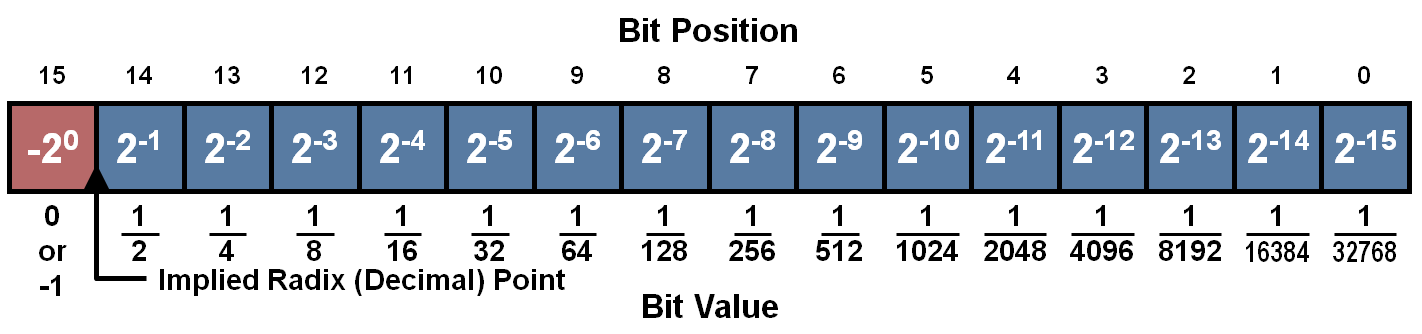
\includegraphics[width=\linewidth]{Figures/Filter/1-15.png}}
\caption{Bit Values of 1.15 Format. Credit: Microchip Developer}
\label{1-15}
\end{figure}

We store the discrete-time output signals from our filter in a similar fashion to our filter coefficients and input samples - in the $1.15$ format. A conversion from a 32-bit multiplication product to a 16-bit output is thus required. We apply the ``round-and-truncate technique'' for the conversion. The 32-bit product from two 16-bit number in 1.15-format follows a very similar bit-value layout to its multipliers. To round and truncate this number, we first discard the most significant bit (by a single left shift on a fixed-sized register) to convert the 32-bit product into a 1.31 format number. Before we discard the 16 least significant bits, we round our current number by adding half of the value of the least significant bit after rounding to the 32-bit number. For example, if we are discarding the least significant 16 bits, we add half of the value of bit 17 (which has a value of $2^16$ in a 32-bit integer) to our output. After rounding the number, we discard the least significant 16 bits and interpret the most significant 16-bits as a number in 1.15 format. Note that this round-and-truncate operation is analogous to rounding and truncating a decimal number. 

With every sample input fed into the system, the filter would carry out $N+1$ Multiply-And-Accumulate (MAC) operations to calculate the convolution product. Given the mathematical mechanics of the FIR filter, we choose to implement an circular buffer to hold input sample signals given the fixed number of MAC operations for each sample as shown in ``Fig.~\ref{circ_buff}''. The write pointer of the circular buffer travels clockwise in accordance to the clockwise layout of the buffer, indicating the index of the latest sample. Given \eqref{fir_conv}, we note that the first filter impulse response term is always multiplied by the latest sample, and the earliest sample received is multiplied by the last filter impulse response term. Hence, the read-pointer of the circular buffer travels in a counter-clockwise fashion, accessing samples received in a reverse chronological order. 


\begin{figure}[!h]
    \centerline{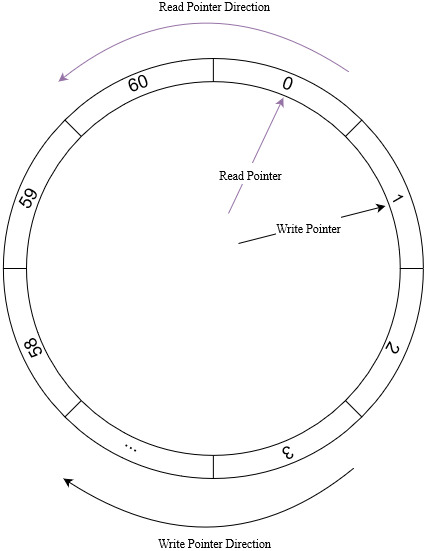
\includegraphics[width=0.85\linewidth]{Figures/Filter/circular_buffer.jpg}}
    \caption{Illustration of Circular Buffer Implementation}
    \label{circ_buff}
\end{figure}

Although not pictured in ``Fig.~\ref{circ_buff}'', both implementations also include a third, "filter impulse response" pointer, indicating the corresponding impulse response term for the sample. This pointer always starts at position 0. As the read pointer travels counter-clockwise by 1, the impulse response pointer travel clockwise (increase) by 1.

\subsection{Software Filter Implementation} \label{software_imp}
The software implementation of our FIR low pass filter takes the form of a C-program running on a Microblaze\textregistered{} microprocessor. The filter C-program is attached in the appendix of this report. The C programming language is a universal programming language, running on microprocessors or desktop processors alike. One relevant distinction of a Microblaze\textregistered{} microprocessor from other platforms lies in the data size of the processor. On a Microblaze\textregistered{} microprocessor, integer values are $32$-bits, while \textit{short} values are only $16$-bits. 

We designed the algorithm of our software implementation as follows:
\begin{algorithm}
    \caption{FIR Filter Software Implementation}
  \begin{algorithmic}[1]
    \REQUIRE Filter impulse response terms available to the program as $Filter$
    \item[\textbf{INPUT:}] Input sample signal in discrete-time (as an array $Sample$)
    \item[\textbf{OUTPUT:}]  Filtered signal in discrete-time
    \STATE \textbf{Initialization} $Read = 0$, $Write = 0$, $Impulse = 0$
    \STATE \textbf{Circular Buffer}: Initialize an array $circ\_buff$ with the same number of elements as the number of impulse response terms
    \WHILE{$Write \leq 60$}
        \STATE $circ\_buff[Write] = 0$
    \ENDWHILE
    \STATE $Write = 0$, $Result = 0$
    \FOR{$index = 0$, $index \leq Sample \; size$}
        \STATE $circ\_buff[Write] = Sample[index]$
        \STATE Set $Read = Write$, $Impulse = 0$
        \WHILE{$Filter \leq 60$}
            \STATE $Result += Filter[Impulse] \times circ\_buff[Read]$
            \STATE $Impulse$++, $Read$--, if $Read = 0$, then set $Read = 60$
        \ENDWHILE
        \STATE Output $Result$ as the output discrete signal at corresponding time
        \STATE $Write$++, if $Write = 60$, then set $Write = 0$
    \ENDFOR
  \end{algorithmic}
\end{algorithm}

Note that $Result$ can either be presented as console text print outputs or collected in an array for later usage.

\begin{figure}[htbp]
    \centerline{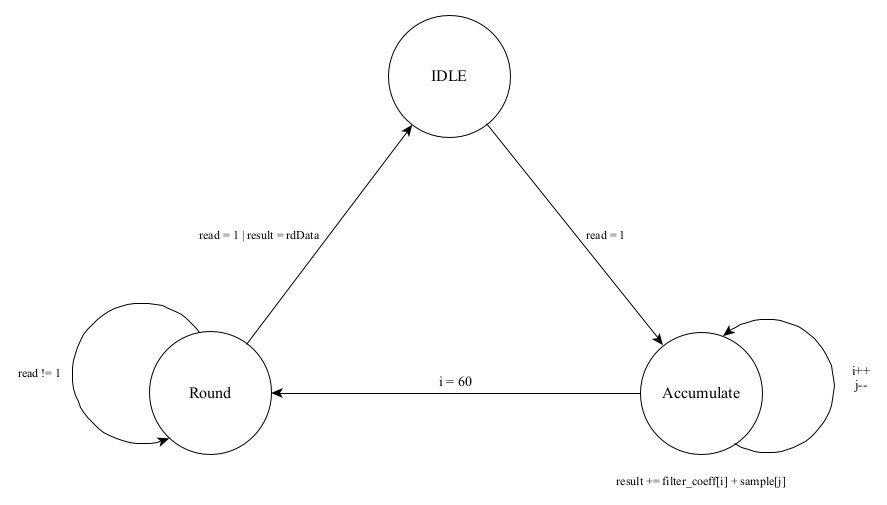
\includegraphics[width=\linewidth]{Figures/Filter/fsm_hardware.jpg}}
    \caption{Logic Diagram of the finite-state Machine}
    \label{fsm}
\end{figure}

\begin{figure*}[htbp]
    \centerline{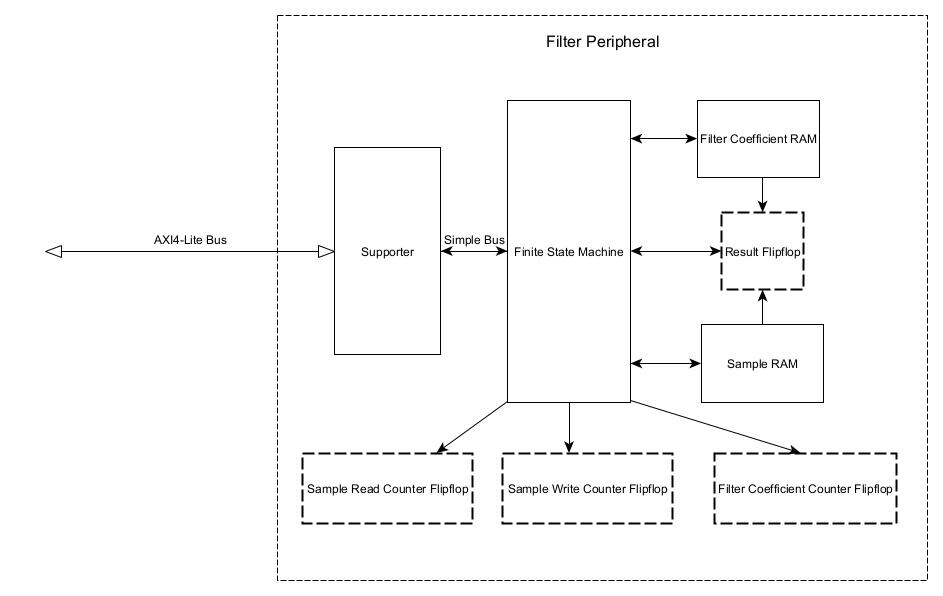
\includegraphics[width=0.8\textwidth]{Figures/Filter/hardware_architecture.jpg}}
    \caption{Illustration of the Hardware Implementation}
    \label{hardware}
\end{figure*}

\subsection{Hardware Filter Implementation} \label{hardware_imp}
The underlying mechanics of the hardware implementation of the FIR low pass filter are very similar to that of the software implementation. The logic for conducting MAC operations are implemented as a Mealy machine in ``Fig.~\ref{fsm}''.

The same circular buffer and read/write counters are implemented in the form of asynchronous-read Random Access Memories (RAM) and flip-flops (as shown in ``Fig.~\ref{hardware})''. 

Note that since the filter peripheral does not contain dedicated memory to store results, the processed sample output must be extracted before the circular buffer accepts another sample. Therefore, the finite state machine will hang in state $round$ until the result is read/extracted by the Microblaze\textregistered{}.



\section{Operation/Testing} \label{testing}

Two sinusoidal test signals are used to test the performance of our FIR low-pass filter: one with frequency within the pass-band, and the other with frequency within the stop-band. Test signals are sampled at $50kHz$ for $0.02s$. Overall, $1000$ sample points per test signal are generated. As shown in ``Fig.~\ref{input_sin}'', the $1kHz$ and $9kHz$ sinusoidal test signals both share a magnitude of $0.9$. We set the maximum amplitude to $0.9$ to avoid potential buffer overflow during MAC operations, given the maximum fraction value $1.15$ format can represent is always less than one, as shown in \eqref{1-15_max}.

\begin{equation}
    N_{max} = 0 \cdot -2^0 + \sum_{i=1}^{15} 2^{-i} \approx 0.9999695
    \label{1-15_max}
\end{equation}

Test signals are discretized by an Excel spreadsheet and imported to both the software and hardware implementation via a C-header file. The details regarding signal import will be discussed in specific implementation subsections below. Filter impulse response terms are imported into both implementations in a similar fashion. We utilize a FIR filter design tool \cite{b2} provided by the instructor to generate the impulse response terms. Specifications regarding the filter are provided in Table \ref{filter_specs} below.

\begin{table*}[!t]
\centering
\caption{Filter Specifications}
    \begin{tabular}{|c|c|c|c|c|c|c|}
    \hline
    \textbf{Filter}&\multicolumn{6}{|c|}{\textbf{Parameters}} \\
    \cline{2-7}
    \textbf{Specifications} & \textbf{$f_{sample}$} & $f_{passband}$ & $f_{stopband}$ & Stopband & Passband & Filter\\
    &&&& Attenuation & Ripple & Order\\
    \hline
    \textbf{Value} & \textbf{\textit{$50kHz$}} & $3.3kHz$ & $6kHz$ & $60dB$ & $8.681mdB$ & 61\\
    \hline
    \end{tabular}
\label{filter_specs}
\end{table*}

\begin{figure}[htbp]
    \centerline{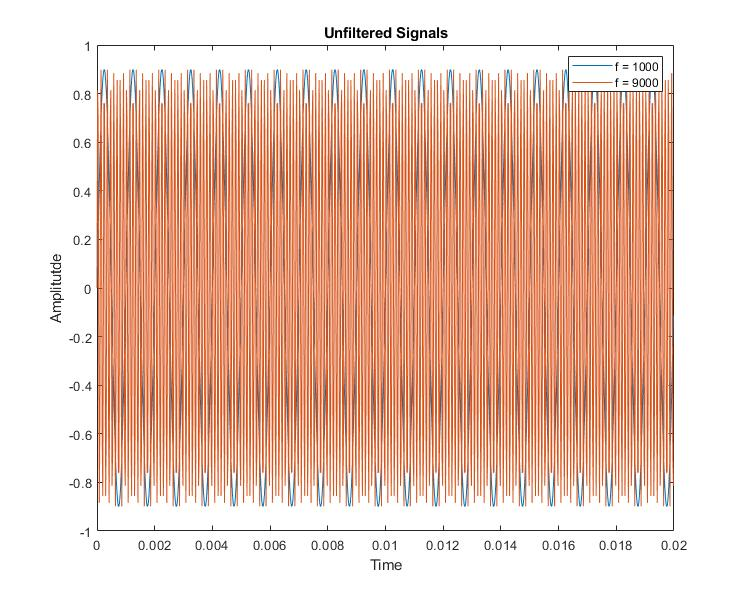
\includegraphics[width=\linewidth]{Figures/Filter/unfiltered_signals.jpg}}
    \caption{Test Sinusoidal Signals}
    \label{input_sin}
\end{figure}

All testing and design are conducted using a Digilent Nexys\texttrademark{} 4 DDR development board. The development board houses a Xilinx\texttrademark{} Artix-7 FPGA chip, and has variable serial connections, peripherals, switches and displays. The Microblaze\textregistered{} processor is implemented using the onboard FPGA, and runs at a clock frequency of 30 Mhz.

\subsection{Software Filter} \label{software_test}

\paragraph{Operation} Implemented according to the algorithm in section \ref{software_imp}, the FIR filter C-program imports two array header files that contain both the filter impulse response terms and the discretized input signals. The program, running on the Microblaze\textregistered{} processor, processes the input signals and records the output signals in an array. The user can choose to either pass the array on for further processing, or output the array via console text print.

\paragraph{Testing} For our low-pass filter implementation, we are mostly interested in the filtering/conversion rate of the filter implementation. The filtering of each discrete time sample is associated with a convolution operation - $N+1$ MAC operations. Timing the MAC operations, therefore, can provide an indicative measurement of the performance of our FIR filter.

To time the MAC operations performed by our software filter, we deviate away from any software timing tools provided either by the compiler or the debugger. Instead, we choose to time the software externally using the circuit elements on the Nexys\texttrademark{}4 DDR board that houses our Microblaze\textregistered{} processor. 

Two PMOD pins are tied to two bits of memory associated with our Microblaze\textregistered{} processor. The C-program writes to these memory prior to any MAC operations, resulting in a $3.3V$ logic high output on the PMOD pins. After the processor complete all MAC operations, the program clears out the memory associated with the output pins, resulting in a logic low output. Using an Oscilloscope, we can easily calculate the amount of time elapsed between the logic high and logic low output, and subsequently time the program. 

\paragraph{Testing Results} The filter program successfully retains the magnitude of the pass-band signal while attenuates that of the stop-band signal. ''Fig.~\ref{output_sin}'' shows the output signal. The results of hardware timing and calculated rates are presented below in Table \ref{software_timing}
\begin{figure}[htbp]
    \centerline{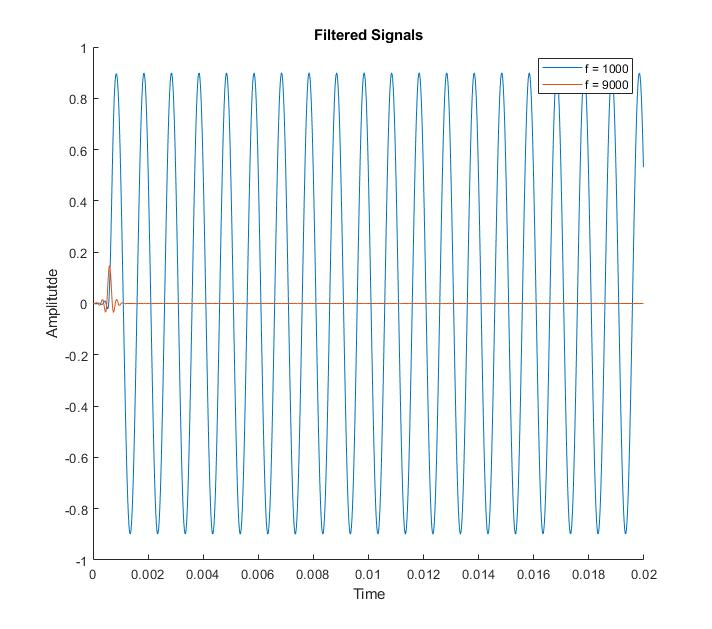
\includegraphics[width=\linewidth]{Figures/Filter/filtered_signals.jpg}}
    \caption{Illustration of the Hardware Implementation}
    \label{output_sin}
\end{figure}

\begin{table}[htbp]
\caption{Software Filter Timing Results}
\begin{center}
\begin{tabular}{|c|c|c|c|c|c|}
\hline
\textbf{Timing}&\multicolumn{5}{|c|}{\textbf{Parameters}} \\
\cline{2-6} 
\textbf{Results} & \textbf{\textit{Total \#}}& \textbf{\textit{Total}}& \textbf{\textit{MAC/s}} & \textbf{\textit{MAC/}}& \textbf{\textit{Samples/}} \\
 & \textbf{\textit{of MAC Ops}} & \textbf{\textit{Time}} & & \textbf{\textit{Sample}} & \textbf{\textit{s}} \\
\hline
Value & $61000$ & $333.4ms$ & $182964$ & $61$ & $2999.4$\\
\hline
\end{tabular}
\label{software_timing}
\end{center}
\end{table}

We also compared the theoretical input lag to the actual filter input lag based on the input/output signals. Input lag results from partial convolution, where the number of impulse response terms exceed the number of total received samples. It can be calculated as shown below in \eqref{input_lag}.
\begin{equation}
    t_{lag} = \frac{\text{FIR Filter Order} \cdot T_{sample}}{2} = \frac{61}{2 \cdot 50kHz} = 0.61ms
    \label{input_lag}
\end{equation}

Experimentally, the (time) distance between the first input signal peak and the first output signal peak of a pass-band signal yields the filter lag. As shown in ``Fig.~\ref{lag}'', the emperically measured lag is $0.6 ms$.

\begin{figure}[htbp]
    \centerline{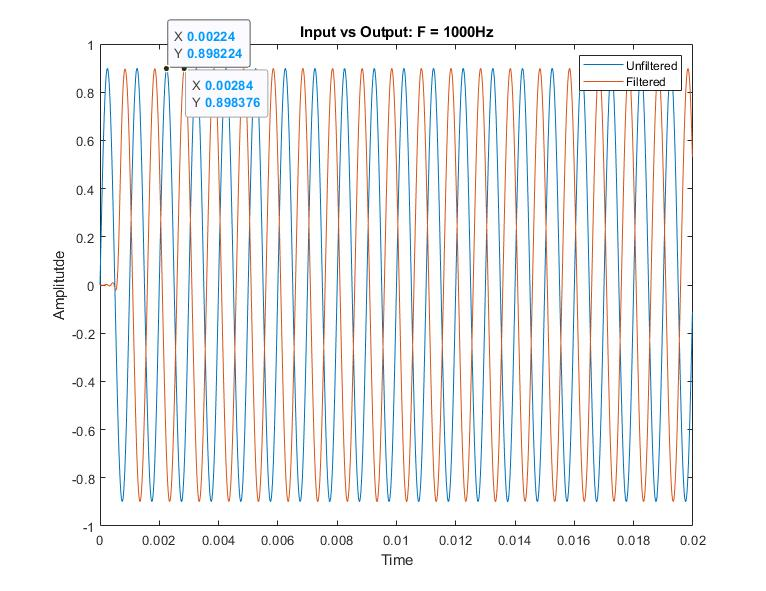
\includegraphics[width=\linewidth]{Figures/Filter/delay_graph.jpg}}
    \caption{Illustration of the Hardware Implementation}
    \label{lag}
\end{figure}

\subsection{Hardware Filter} \label{hardware_test}

\paragraph{Operation}
Functionally, the hardware filter implementation is identical to its software counterpart. The hardware FIR filter is implemented as an AXI4-Lite peripheral using the same Xilinx\textregistered \;Field Programmable Gate Array (FPGA) board. The filter peripheral communicates with the Microblaze\textregistered{} processor using the AXI4-Lite bus. Based on the hardware and logic design given in section \ref{hardware_imp}, we constructed and realized the hardware implementation using our Nexys\texttrademark{}4 DDR board. The Verilog description of the hardware peripheral is available in the appendix of this report.

To use this peripheral in an isolated fashion, an interface program running on the Microblaze\textregistered{} microprocessor is required. This program serves both as an filter interface that provides the impulse response terms and an Analog-to-Digital Converter (ADC), which provides input samples to the peripheral in discrete time. In addition, this program collects the output signals from the filter peripheral.

Analogous to how the software filter operates, the interface program access the peripheral first to write all filter impulse response terms to the dedicated, asynchronous-read RAM. The program then zeros out the sample-dedicated RAM to prepare for convolution operations. The interface program writes in discrete-time samples one at a time while extracting the processed output. After each sample-write operation, the program hangs the sample-writing process and continuously polls the peripheral until the filtered results is received.

\paragraph{Testing and Results} The filtered results obtained from the hardware peripheral are identical to those produced from the software implementation. However, the hardware filter peripheral is significantly faster at processing samples, as shown in Table \ref{hardware_timing}.


\begin{table}[htbp]
\caption{Hardware Filter Timing Results}
\begin{center}
\begin{tabular}{|c|c|c|c|c|}
\hline
\textbf{Timing}&\multicolumn{4}{|c|}{\textbf{Parameters}} \\
\cline{2-5} 
\textbf{Results} & \textbf{\textit{Total \#}}& \textbf{\textit{Total}}& \textbf{\textit{MAC/s}} & \textbf{\textit{Samples/}} \\
 & \textbf{\textit{of MAC Ops}} & \textbf{\textit{Time}} &  & \textbf{\textit{s}} \\
\hline
Value & $61000$ & $4.8344ms$ & $12617905$ & $206851$\\
\hline
\end{tabular}
\label{hardware_timing}
\end{center}
\end{table}

\paragraph{Software Bottleneck within Hardware Implementations} Given the layout of our finite state machine, when the filter remains in the "accumulate" state, every MAC operation takes exactly 1 clock cycle to complete. Given the $30MHz$ clock frequency of our Microblaze \textregistered microprocessor, our maximum $MAC/s$ rate should approach the Microblaze clock frequency, $30M$ MAC$/s$. In reality, our hardware filter is only able to achieve a maximum rate of $12M$ MAC$/s$. 

Upon further examination, we discover that with every input sample, the finite state machine hangs in the "round" state and wait for the interface program to collect filter output data. Given our implementation, our interface program continuously polls the hardware filter until the MAC operations are complete. We hypothesize that reducing the software polling time - therefore reducing the finite state machine hang-time - would increase the hardware filter processing time as a result. Moreover, because our interface also serves as an ADC, increasing the ``conversion rate'' of our interface program can hypothetically boost the sample processing rate.

To reduce the software polling time and increase the sample-writing rate, we introduce loop unwinding, an optimization technique that sacrifices space complexity for time complexity. Programs written in C are translated to machine instructions in assembly by the compiler. During the translation process, complex branching commands are introduced. A loop-unwinded program conducts multiple loop operations in one sitting before checking the loop condition, thus avoiding extra branching commands. Given our finite state machine needs a set of amount of time to conduct MAC operations, we can safely loop-unwind our interface program and conduct a set number of polling operations without checking the loop condition that resets the finite state machine back to "idle" state. Overall, we see a speed increase in our filter performance after eliminating some branching commands from the interface program. Table \ref{loop_unwind} shows the consequent MAC rate boosts from successive loop-unwinding.

\begin{table}[htbp]
\caption{Hardware Filter Loop-unwinded}
\begin{center}
\begin{tabular}{|c|c|c|c|}
\hline
\textbf{Timing}&\multicolumn{3}{|c|}{\textbf{Specifics}} \\
\cline{2-4} 
\textbf{Results} & \textbf{\textit{Elasped}} & \textbf{\textit{MAC/s}}& \textbf{\textit{Speed Increase}}\\
 & \textbf{\textit{Time}} & & (\%)\\
\hline
Control & $4.8344ms$ & $12617905$ & NA\\
\hline
1x Polling & & &\\
-loop Unwinded & $4.1340ms$ & $14755684$ & $16.94\%$\\
\hline
2x Polling & & &\\
-loop Unwinded & $3.8838ms$ & $15706267$ & $24.48\%$ \\
\hline
4x Polling & & &\\
-loop \& 2x ADC & $3.0760ms$ & $19830949$ & $57.17\%$\\
-loop Unwinded & & & \\
\hline
\end{tabular}
\label{loop_unwind}
\end{center}
\end{table}


\section{Discussions and Conclusions} \label{conclusion}

Though both implementations use identical logic and accomplish the same task, it is clear that the hardware implementation filters signals at a drastically faster rate. The software implementation can process signals around a rate of $3k$ MAC$/s$, while its hardware counterpart filters signals at around $207k$ MAC$/s$,This drastic speed difference could be attributed to the nature of software written in a high-level programming languages like C. The software implementation, on the surface level, carries out the same operations as the hardware implementation. Yet when the program is compiled into machine instructions, operations such as array-memory allocation and loop branching collectively consume much more time. Inversely, the hardware implementation eliminates memory allocation time by implementing dedicated storage, and cuts down on loop branching with a finite state machine, which constraints the maximum loop branching time to one clock cycle. 

Given the widespread nature of FIR filters, it is strongly recommended for engineers to implement dedicated hardware filters. As demonstrated by this report, software implementations of FIR filters are simply too inefficient comparing to hardware implementations.


\begin{thebibliography}{00}
\bibitem{b1} A. V. Oppenheim, J. Buck, M. Daniel, A. S. Willsky, S. H. Nawab, and A. Singer, ``Signals and Systems,'' Prentice Hall, 2nd Edition, 1997.
\bibitem{b2} LabVIEW Filter Design Tool, ESE-465: Digital Systems Laboratory, Washington University in St. Louis, 2022
\bibitem{b3} When is loop unwinding effective?\\ https://stackoverflow.com/questions/190681/when-is-loop-unwinding-effective
\end{thebibliography}

\newpage
\onecolumn
\section{Appendix: Program Source Code in C}
\subsection{Software Implementation}
\lstinputlisting[language=C]{Code/Filter/Filter.c}
\subsection{Hardware Peripheral Verilog}
\lstinputlisting[language=Verilog]{Code/Filter/Axi4LiteFilter.v}
\subsection{Hardware Filter Interface Program}
\lstinputlisting[language=C]{Code/Filter/filter_peripheral.c}
\subsection{Sample Input Header File}
\lstinputlisting[language=C]{Code/Filter/sample.h}
\end{document}
